\documentclass[11pt]{book}

%%%%%%%%%%%%%%Include Packages%%%%%%%%%%%%%%%%%%%%%%%%%%
\usepackage{xcolor}
\usepackage{mathtools}
\usepackage[legalpaper, total={6in, 8in}, margin=1.25in]{geometry}
\usepackage{amsmath}
\usepackage{amssymb}
\usepackage{paralist}
\usepackage{rsfso}
\usepackage{amsthm}
\usepackage{wasysym}
\usepackage[inline]{enumitem}   
\usepackage{hyperref}
\usepackage{tocloft}
\usepackage{wrapfig}
\usepackage{titlesec}
\usepackage{colortbl}
\usepackage{stackengine} 
\usepackage{csvsimple}
\usepackage{listings}
%%%%%%%%%%%%%%%%%%%%%%%%%%%%%%%%%%%%%%%%%%%%%%%%%%%%%%%%



%%%%%%%%%%%%%%%Code%%%%%%%%%%%%%%%%%%%%%%%%%%%%%%%%%%%%%
\definecolor{codegreen}{rgb}{0,0.6,0}
\definecolor{codegray}{rgb}{0.5,0.5,0.5}
\definecolor{codepurple}{rgb}{0.58,0,0.82}
\definecolor{backcolour}{rgb}{0.95,0.95,0.92}

\lstdefinestyle{mystyle}{
    backgroundcolor=\color{backcolour},   
    commentstyle=\color{codegreen},
    keywordstyle=\color{magenta},
    numberstyle=\tiny\color{codegray},
    stringstyle=\color{codepurple},
    basicstyle=\ttfamily\footnotesize,
    breakatwhitespace=false,         
    breaklines=true,                 
    captionpos=b,                    
    keepspaces=true,                 
    numbers=left,                    
    numbersep=5pt,                  
    showspaces=false,                
    showstringspaces=false,
    showtabs=false,                  
    tabsize=2
}
%%%%%%%%%%%%%%%%%%%%%%%%%%%%%%%%%%%%%%%%%%%%%%%%%%%%%%%%




%%%%%%%%%%%%%%%Chapter Setting%%%%%%%%%%%%%%%%%%%%%%%%%%
\definecolor{gray75}{gray}{0.75}
\newcommand{\hsp}{\hspace{20pt}}
\titleformat{\chapter}[hang]{\Huge\bfseries}{\thechapter\hsp\textcolor{gray75}{$\mid$}\hsp}{0pt}{\Huge\bfseries}
%%%%%%%%%%%%%%%%%%%%%%%%%%%%%%%%%%%%%%%%%%%%%%%%%%%%%%%%

%%%%%%%%%%%%%%%%%Theorem environments%%%%%%%%%%%%%%%%%%%
\newtheoremstyle{break}
  {\topsep}{\topsep}%
  {\itshape}{}%
  {\bfseries}{}%
  {\newline}{}%
\theoremstyle{break}
\theoremstyle{break}
\newtheorem{axiom}{Axiom}
\newtheorem{thm}{Theorem}[section]
\renewcommand{\thethm}{\arabic{section}.\arabic{thm}}
\newtheorem{lem}{Lemma}[thm]
\newtheorem{prop}[lem]{Proposition}
\newtheorem{corL}{Corollary}[lem]
\newtheorem{corT}[lem]{Corollary}
\newtheorem{defn}{Definition}[corL]
\newenvironment{indEnv}[1][Proof]
  {\proof[#1]\leftskip=1cm\rightskip=1cm}
  {\endproof}
%%%%%%%%%%%%%%%%%%%%%%%%%%%%%%%%%%%%%%%%%%%%%%%%%%%%%%


%%%%%%%%%%%%%%%%%%%%%%%Integral%%%%%%%%%%%%%%%%%%%%%%%
\def\upint{\mathchoice%
    {\mkern13mu\overline{\vphantom{\intop}\mkern7mu}\mkern-20mu}%
    {\mkern7mu\overline{\vphantom{\intop}\mkern7mu}\mkern-14mu}%
    {\mkern7mu\overline{\vphantom{\intop}\mkern7mu}\mkern-14mu}%
    {\mkern7mu\overline{\vphantom{\intop}\mkern7mu}\mkern-14mu}%
  \int}
\def\lowint{\mkern3mu\underline{\vphantom{\intop}\mkern7mu}\mkern-10mu\int}
%%%%%%%%%%%%%%%%%%%%%%%%%%%%%%%%%%%%%%%%%%%%%%%%%%%%%%



\newcommand{\R}{\mathbb{R}}
\newcommand{\N}{\mathbb{N}}
\newcommand{\Z}{\mathbb{Z}}
\newcommand{\Q}{\mathbb{Q}}
\newcommand{\C}{\mathbb{C}}
\newcommand{\T}{\mathcal{T}}
\newcommand{\M}{\mathcal{M}}
\newcommand{\Symm}{\text{Symm}}
\newcommand{\Alt}{\text{Alt}}
\newcommand{\Int}{\text{Int}}
\newcommand{\Bd}{\text{Bd}}
\newcommand{\Power}{\mathcal{P}}
\newcommand{\ee}[1]{\cdot 10^{#1}}
\newcommand{\spa}{\text{span}}
\newcommand{\sgn}{\text{sgn}}
\newcommand{\degr}{\text{deg}}
\newcommand{\pd}{\partial}
\newcommand{\that}[1]{\widetilde{#1}}
\newcommand{\lr}[1]{\left(#1\right)}
\newcommand{\vmat}[1]{\begin{vmatrix} #1 \end{vmatrix}}
\newcommand{\bmat}[1]{\begin{bmatrix} #1 \end{bmatrix}}
\newcommand{\pmat}[1]{\begin{pmatrix} #1 \end{pmatrix}}
\newcommand{\rref}{\xrightarrow{\text{row\ reduce}}}
\newcommand{\txtarrow}[1]{\xrightarrow{\text{#1}}}
\newcommand\oast{\stackMath\mathbin{\stackinset{c}{0ex}{c}{0ex}{\ast}{\Circle}}}


\newcommand{\note}{\color{red}Note: \color{black}}
\newcommand{\remark}{\color{blue}Remark: \color{black}}
\newcommand{\example}{\color{green}Example: \color{black}}
\newcommand{\exercise}{\color{green}Exercise: \color{black}}

%%%%%%%%%%%%%%%%%%%%%%Roman Number%%%%%%%%%%%%%%%%%%%%%%%
\makeatletter
\newcommand*{\rom}[1]{\expandafter\@slowromancap\romannumeral #1@}
\makeatother
%%%%%%%%%%%%%%%%%%%%%%%%%%%%%%%%%%%%%%%%%%%%%%%%%%%%%%%%%

%%%%%%%%%%%%table of contents%%%%%%%%%%%%%%%%%%%%%%%%%%%%
\setlength{\cftchapindent}{0em}
\cftsetindents{section}{2em}{3em}

\renewcommand\cfttoctitlefont{\hfill\huge\bfseries}
\renewcommand\cftaftertoctitle{\hfill\mbox{}}

\setcounter{tocdepth}{2}
%%%%%%%%%%%%%%%%%%%%%%%%%%%%%%%%%%%%%%%%%%%%%%%%%%%%%%%%%


%%%%%%%%%%%%%%%%%%%%%Footnotes%%%%%%%%%%%%%%%%%%%%%%%%%%%
\newcommand\blfootnote[1]{%
  \begingroup
  \renewcommand\thefootnote{}\footnote{#1}%
  \addtocounter{footnote}{-1}%
  \endgroup
}
%%%%%%%%%%%%%%%%%%%%%%%%%%%%%%%%%%%%%%%%%%%%%%%%%%%%%%%%%

%%%%%%%%%%%%%%%%%%%%%Section%%%%%%%%%%%%%%%%%%%%%%%%%%%%%
\makeatletter
\def\@seccntformat#1{%
  \expandafter\ifx\csname c@#1\endcsname\c@section\else
  \csname the#1\endcsname\quad
  \fi}
\makeatother
%%%%%%%%%%%%%%%%%%%%%%%%%%%%%%%%%%%%%%%%%%%%%%%%%%%%%%%%%

%%%%%%%%%%%%%%%%%%%%%%%%%%%%%%%%%%%Enumerate%%%%%%%%%%%%%%
\makeatletter
% This command ignores the optional argument 
% for itemize and enumerate lists
\newcommand{\inlineitem}[1][]{%
\ifnum\enit@type=\tw@
    {\descriptionlabel{#1}}
  \hspace{\labelsep}%
\else
  \ifnum\enit@type=\z@
       \refstepcounter{\@listctr}\fi
    \quad\@itemlabel\hspace{\labelsep}%
\fi}
\makeatother
\parindent=0pt
%%%%%%%%%%%%%%%%%%%%%%%%%%%%%%%%%%%%%%%%%%%%%%%%%%%%%%%%%%


\begin{document}

	\begin{titlepage}
		\begin{center}
			\vspace*{1cm}
			\Huge \color{red}
				\textbf{Lab 4 Report}\\
			\vspace{0.5cm}			
			\Large \color{black}
				Math 391 - Introduction to Modern Physics Lab\\
				Professor Wayne Lau\\	
				University of Michigan\\
			\vspace{3cm}

			
\includegraphics[scale=0.8]{Jinyan'sQuestion.pdf}
			
			
			\vspace{5cm}
			\LARGE
				\textbf{Jinyan Miao}\\
				\hfill\break
				\LARGE Fall 2022\\
			\vspace{1cm}

		\vspace*{\fill}
		\end{center}			
	\end{titlepage}


\newpage
\tableofcontents
\addtocontents{toc}{~\hfill\textbf{Page}\par}


\setcounter{chapter}{4}
\chapter*{Lab 4 - Diffraction and Interference}
\section{Introduction}
Diffraction and interference are key features in the propagation of waves. If waves are in phase, the intensity is enhanced, and if waves are out of phase, the intensity is reduced. The single slit experiment verifies the wave property of light by demonstrating the phenomenon of diffraction and interference of light waves. \\

In the single slit experiment, a parallel light beam of wavelength $\lambda$ is shone through a single slit of width $a$. The diffraction property of light causes the light to propagate in different directions making angles $-\pi/2\leq \theta\leq \pi/2$ with respect to the normal of the slit. The intensity recorded at a distant screen illuminated by the slit is given by the following:
\begin{align*}
I = I_0 \left( \frac{\sin(\alpha)}{\alpha}\right)^2
\end{align*}
where $I_0$ is the intensity of the central maximum, and $\alpha$ is defined by the following:
\begin{align*}
\alpha = \frac{\pi a}{\lambda} \sin(\theta)
\end{align*}
From the simple geometry of this problem, the dark bands on the screen are characterized by the following equation, where we denote the distance from the dark bands to the central maximum as $x$, and we denote the distance between the screen and the slit as $L$:
\begin{align}
\frac{x}{L} = \tan(\theta) \approx \sin(\theta) =  \frac{n\lambda}{a} \qquad\qquad\qquad \text{for small } n \in \N
\end{align}
here we utilize the small angle approximation as we assume that $L \gg x$. Hence the width of the slit can be determined by the following:
\begin{align}
\qquad\qquad a = \frac{n \lambda L}{x} \ \quad\qquad\qquad\qquad\qquad \text{for small } n \in \N
\end{align}
Here (4.2) holds as long as the small angle approximation can be used, hence we can see a narrow band of light on the screen with intensity minima at uniform intervals. Let $\Delta x$ denote the distance between the minima, (4.2) becomes the following:
\begin{align}
a = \frac{\lambda L }{\Delta x}
\end{align}
Now for multiple slits of uniform spacing, let $d$ denote the spacing between the slits, the bright fringes on the screen are characterized by the following, where we denote the distance from the central maximum to the bright fringe as $x$:
\begin{align}
\frac{x}{L}=\tan(\theta) \approx \sin(\theta) =\frac{ m \lambda}{d}  \qquad\qquad\qquad \text{for small }m \in \N
\end{align}
utilizing a similar argument to that of dark fringes illuminated by the single slit, one finds that we have the following for $\Delta x$ being the distance between bright fringes illuminated by the multiple slits of equal spacing $d$:
\begin{align}
d = \frac{\lambda L}{\Delta x}
\end{align}

The wave property of light plays key roles in observing and measuring microscopic objects. In Lab 4 of Physics 391, we perform the single/multiple slit experiments and use the wave properties of light to measure the thickness of a wire and Han's hair. We also use the Michelson Interferometer to measure the thickness of a microscope slide and a cover glass.

\hfill\break
\hfill\break
\section{Experimental setup}
Lab 4 of Physics 391 is split into three parts. In part one of Lab 4, we performed the single slit experiment to measure the width of a slit by using light of three different wavelengths: $405\, nm$ (blue), $532\, nm$ (green), and $635\, nm$ (red). By Babinet's Principle, the physics and the results remain unchanged if one replaces the slit of width $a$ with an obstructing line of equal width. Therefore, we can also use (4.3) to measure the width of an object. We then measured the thickness of a thin straight wire and the thickness of Chi Han's hair. In this part, the object of interest (the slit, wire, and hair) was held fixed on top of a metal shroud, and a light beam was shone at the object, producing a pattern at the bottom plate of the metal shroud. Small strips of luminescent dots were used as a reference for the distance scale. We then took photos of the pattern and measured the distance between the intensity minima in the pattern using rulers in Adobe Photoshop. \\

In the second part of Lab 4, we observed diffraction patterns generated by square mesh, helical lamp filament, and a circular hole in aluminum foil. Then we measured the pattern spacing generated by a diffraction grating by employing a similar procedure given in the first part of Lab 4, the spacing between fringes was calculated via (4.5).\\

In the third part of Lab 4, we measure the thicknesses of a microscope slide and a cover glass using the Michelson interferometer, the procedure for operating the Michelson interferometer is written in the Lab manual, we then analyze our data (the distance of the first four intensity minima on either side of normal incidence) through Microsoft Excel to fit the interference pattern. 
 

\section{Analyzing the data}
\subsection{Width and spacing measurement experiments}
The calculated width (unit in $mm$) of the slit, wire, and hair, and the calculated spacing (unit in $mm$) for the gratings, from the three incident beams of different wavelengths, are presented as the followings:
\begin{center}
\begin{tabular}{|c|c|c|c|c|c|}
\hline
 & 635 nm light & 532 nm light & 405 nm light & mean & st. dev.\\
\hline
single slit & 0.0495 & 0.0507 & 0.0502 & 0.0501 & 0.0006\\
\hline
wire & 0.0241 & 0.0239 & 0.0253 & 0.0245 & 0.0008\\
\hline
Han's hair & 0.0804 & 0.0766 & - & 0.0785 & 0.0026 \\
\hline
gratings & 0.00995 & 0.00994 & 0.0100 & 0.00997 &  0.00003\\
\hline
\end{tabular}
\end{center}
The width of the single slit is estimated to be $50.1\, \mu m$, with a standard deviation of $0.6\, \mu m$. \\
The width of the wire is estimated to be $24.5\, \mu m$, with a standard deviation of $0.8\, \mu m$. Note that the designed width of the thin wire (Nifethal 70, p/n PX000224) is $23\, \mu m$, here we see that:
\begin{align*}
\frac{(23\, \mu m)-(24.5\mu m)}{0.8\,\mu m} = -1.857
\end{align*}
so the designed width is within $2$ standard deviations from our experiment data, which implies that the designed value is statistically well predicted. The thickness of Han's hair is estimated to be $78.5\, \mu m$, with a standard deviation of $2.6\, \mu m$. Note that the estimation of the thickness of hair has a higher variation mainly because the sample size is smaller. We did not have the $405\, nm$
measurement for hair because the distance between the minima for the blue light is too hard to be measured as the hair is thicker than other materials. For the gratings, the mean spacing between the slits is estimated to be $9.97\, \mu m$, with a standard deviation of $0.03\,\mu m$. The gratings in use are designed to have line densities of $100$ per millimeter, which gives a uniform spacing of around $10\, \mu m$. Note that we have:\begin{align*}
\frac{(10\,\mu m )- (9.97\, \mu m)}{0.03\,\mu m} = 1
\end{align*}
Hence we see that the designed spacing is within $1$ standard deviation from our experimental data, which implies the designed spacing is well predicted by our experimental results.\\





\newpage 
\subsection{Michelson interferometer experiment}For the Michelson interferometer experiment, the best-fit interference patterns for the cover glass and the slide are shown in the followings:
\begin{center}
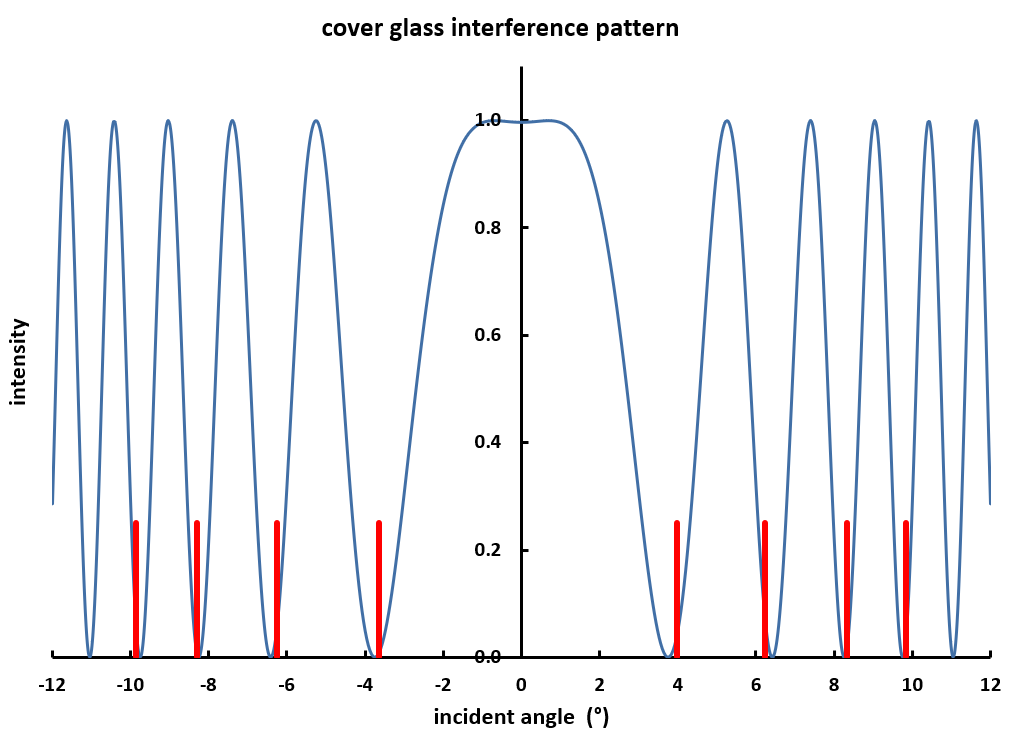
\includegraphics[scale=0.55]{coverGlass.png}\\
\hfill\break
\hfill\break
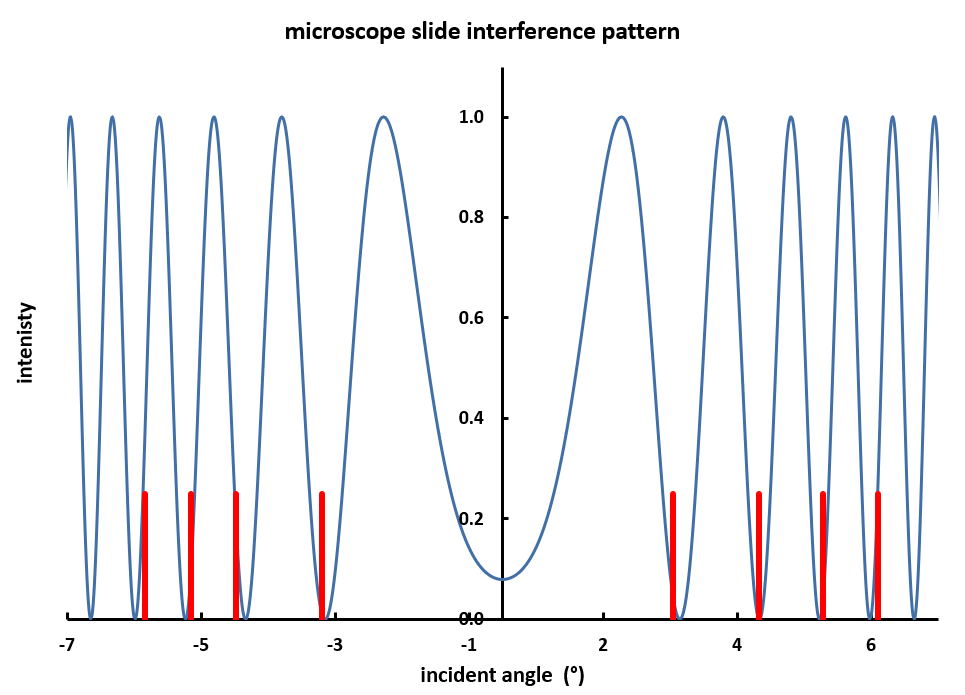
\includegraphics[scale=0.55]{slide.png}
\end{center}
In the figures, the red bands represent the positions of the dark bands that we measured in the experiment, and the blue curves represent the best-fitted interference model. Here we define:
\begin{align*}
\Delta \coloneqq \sum_{n=1}^{8}(\theta_n - \theta_{1,n})^2
\end{align*}
where $\{\theta_n\}$ are the incident angles calculated from the eight minima in the experimental data, and the $\{\theta_{1,n}\}$ are the incident angles calculated from the minima in the best-fitted interference model. Here $\theta_n, \theta_{1,n}$ are measured in degrees. The fitted parameters are given by the followings:
\begin{center}
\begin{tabular}{|c|c|c|c|}
\hline 
 & $\Delta$ & $d$ & $\phi$\\
\hline
Cover glass & $0.1520$ & $0.2228\, nm$ & $0.1110$\\
\hline
Slide & $0.0798$ & $0.7864\, nm$ & $2.5716$\\
\hline
\end{tabular}
\end{center}
where $d$ is the best-fitted thickness of the object, and $\phi$ is a free parameter corresponding to the phase angle of the two interferometer beams, and they are related via the following equation according to the Lab Manual:
\begin{align*}
\theta_{m,1}=\sqrt{\frac{n'}{n'-1}\frac{\lambda}{2d} \left( 2m-1 +\frac{\phi}{\pi}\right)}
\end{align*}
where $\lambda$ is the wavelength of the incident light, $n'$ is the index of refraction of the glass, and $\theta_{m,1}$ is the best-fitted incident angle of the $m$-th minima from the central fringe. The fitting process is done by minimizing $\Delta$ via different values of $d$ and $\phi$. In this process, we can only estimate the error in this experiment through $\Delta$, and the conclusion we can get from $\Delta$ is that the estimation for the thickness of the slide is better than the estimation of the thickness of the cover glass. Note that the cover glass is designed to have a thickness of $0.2 \, mm$, and our result differs from this value by $11.4\%$. The slide is designed to have a thickness of $1\, nm$, and our result differs from this value by $21.4\%$. It is not clear whether our experimental result agrees with the predicted values as the sample size is too small for both the cover glass (sample size$=$1) and the slide (sample size$=$1). \\


\subsection{Other observations in the experiment}
Lastly, we briefly describe what we observed for the diffraction patterns of the square mesh, helical lamp filament, and circular hole in aluminum foil.\\



For the square mesh, the illuminated pattern on the bottom plate consists of two thick bands of light crosses orthogonally to each other. At their intersection, there are nine bright spots arranged in a square-matrix shape, and around their intersection, there are also many smaller less-bright spots. The two thick bands consist of small thick vertical bands, similar to the shape of the old fashion metal watch band. The illuminated square mesh produces this pattern because the mesh is like a combination of two gratings orthogonal to each other. 
\begin{center}
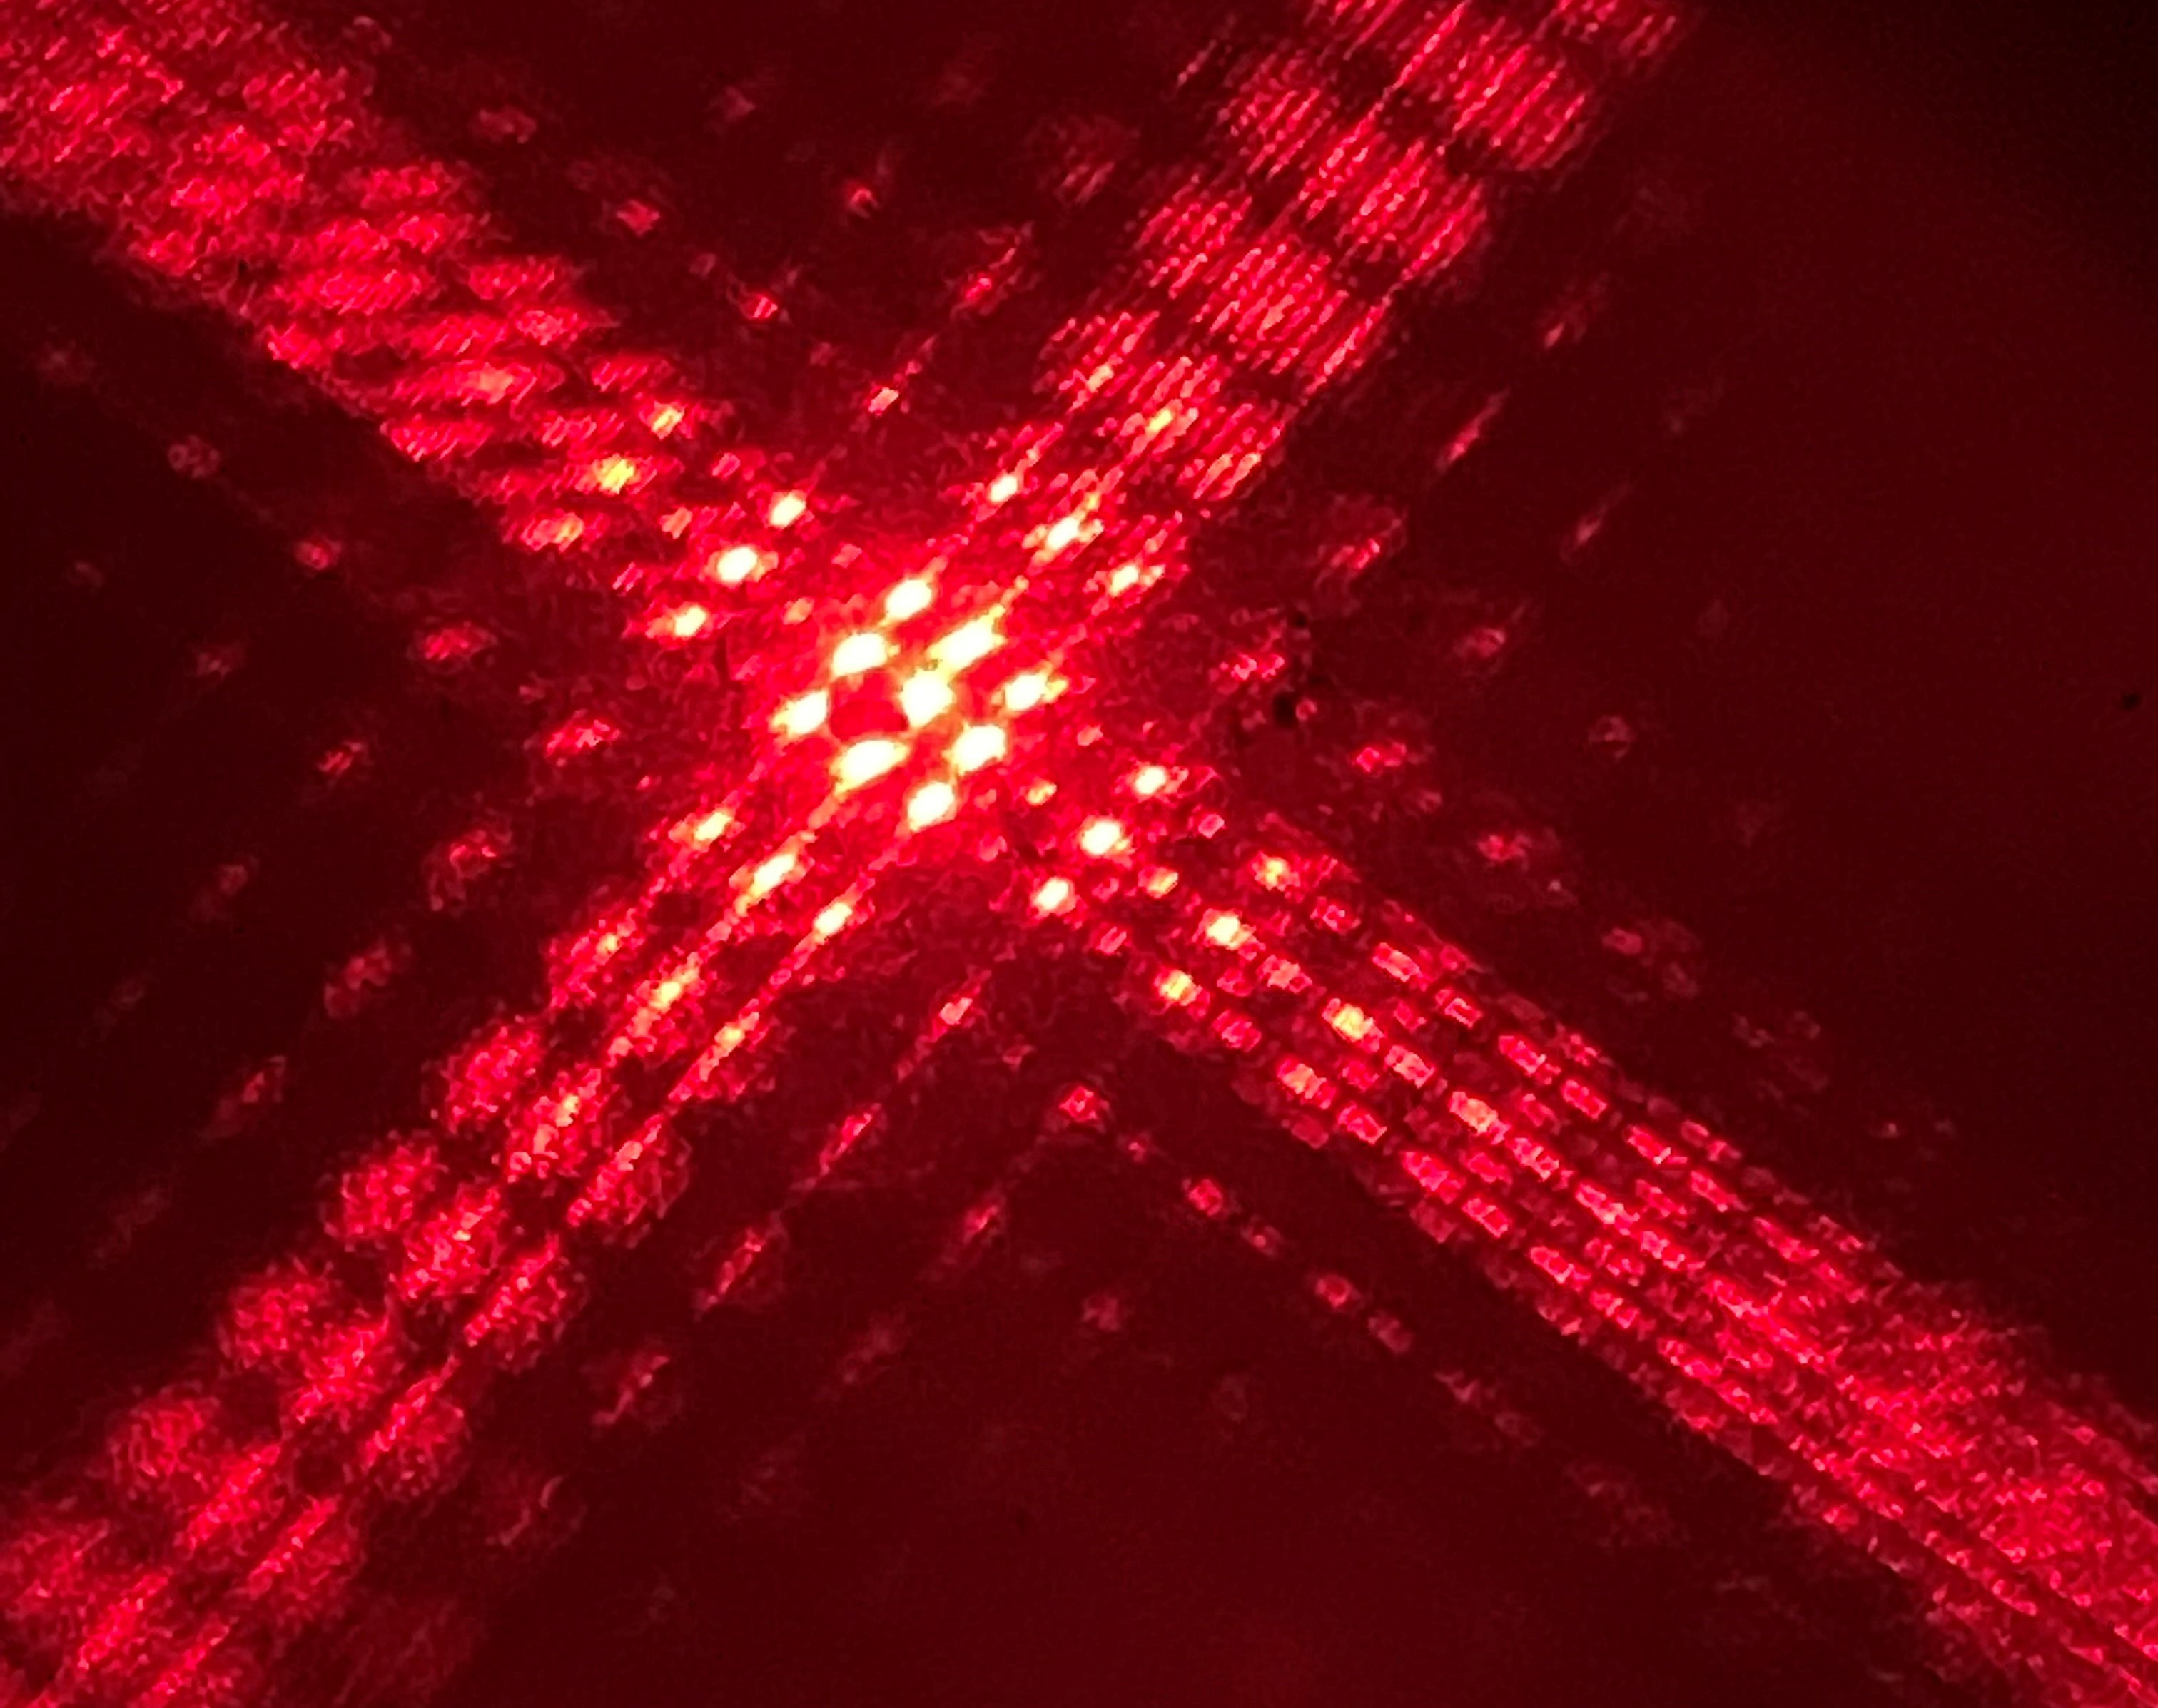
\includegraphics[scale=0.08]{mesh.jpg}
\end{center}


For the helical lamp filament, the illuminated pattern on the bottom plate consists of two thin straight light bands intersecting at an angle. Each thin band is similar to that produced by the single slit. The region between the two thin bands has some blurred and curved fringes. 
\begin{center}
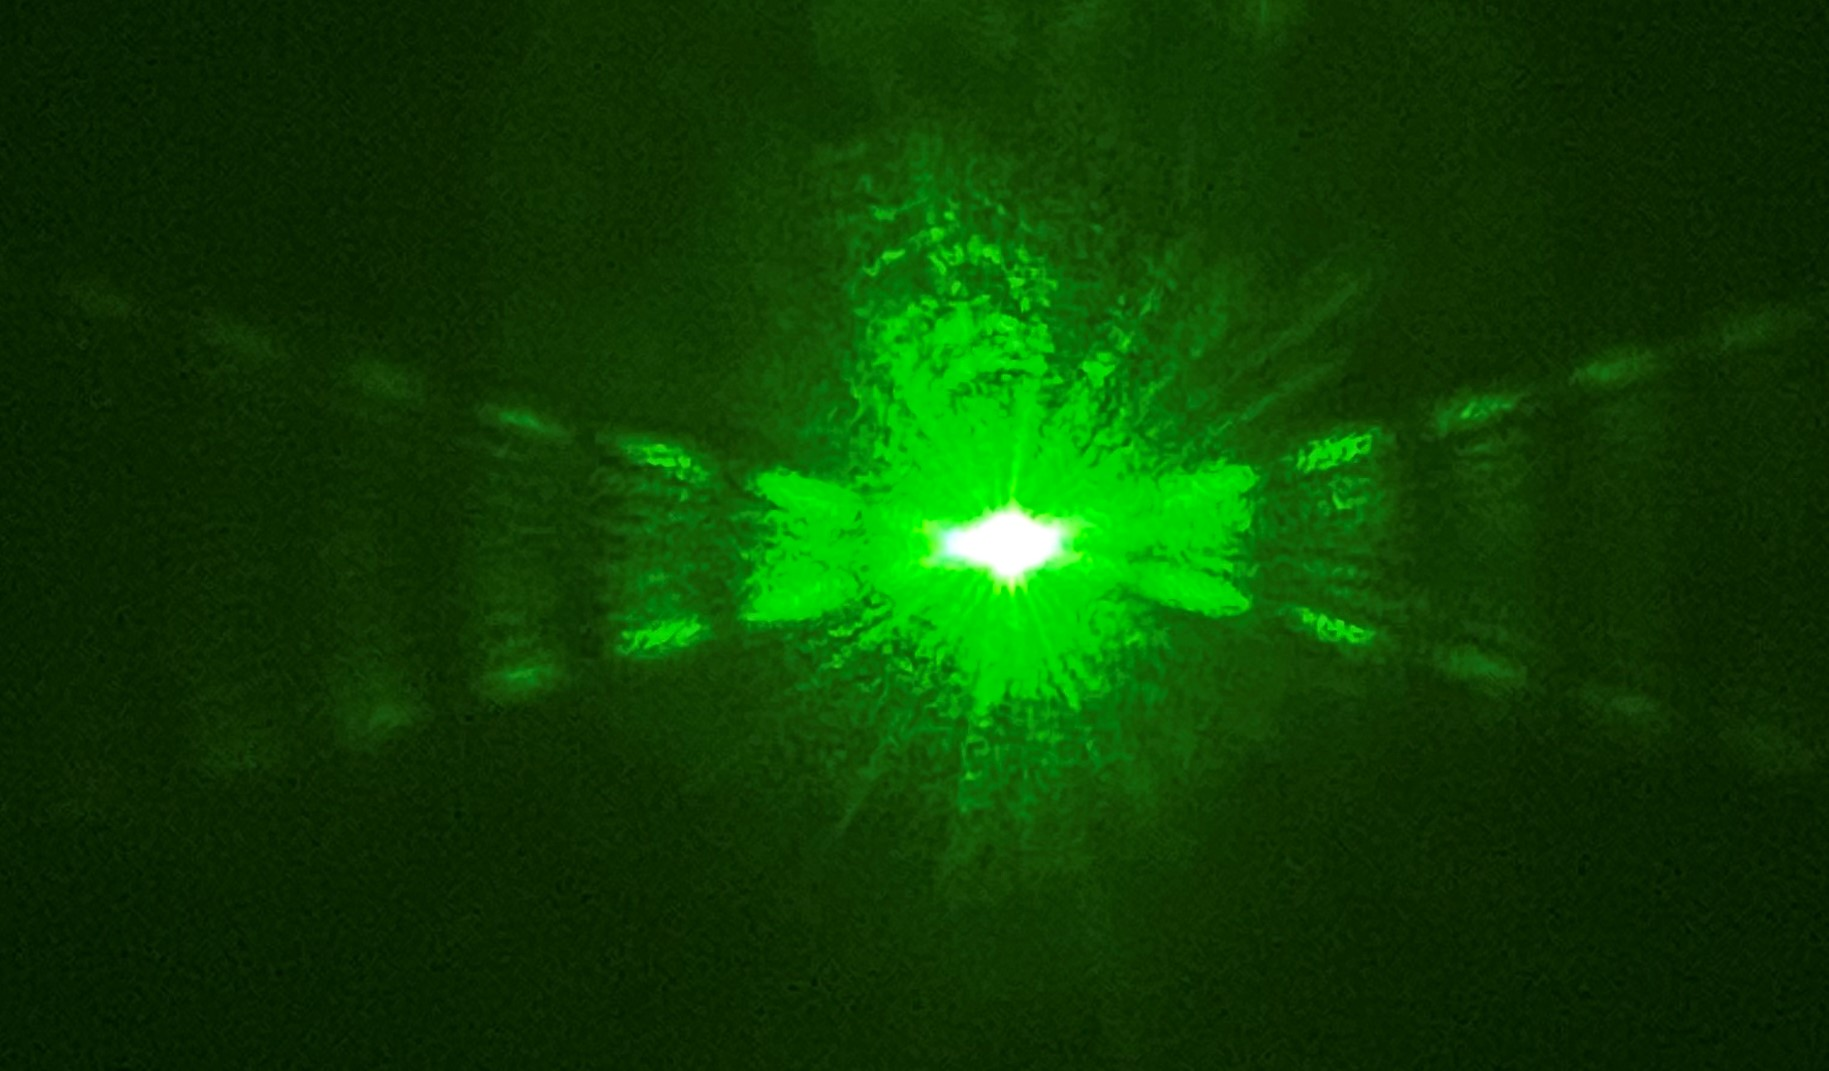
\includegraphics[scale=0.13]{helix.jpg}
\end{center}

For the circular hole in an aluminum foil, we see an illuminated pattern similar to the water wave pattern produced by a large stone falling into the water. That is we see approximately circular concentric bright bands centered at the central maximum. These bands are not in perfect circles because the hole in the aluminum that we made is not a perfect circle. Compared to the pattern created by a single slit, which can be viewed as a one-dimensional light band, the pattern created by the hole is two-dimensional. This makes sense because the light that passes through the hole is diffracted along both axes in the two-dimensional plane, while the light that passes through the slit is only diffracted along a single axis normal to the orientation of the slit. 
\begin{center}
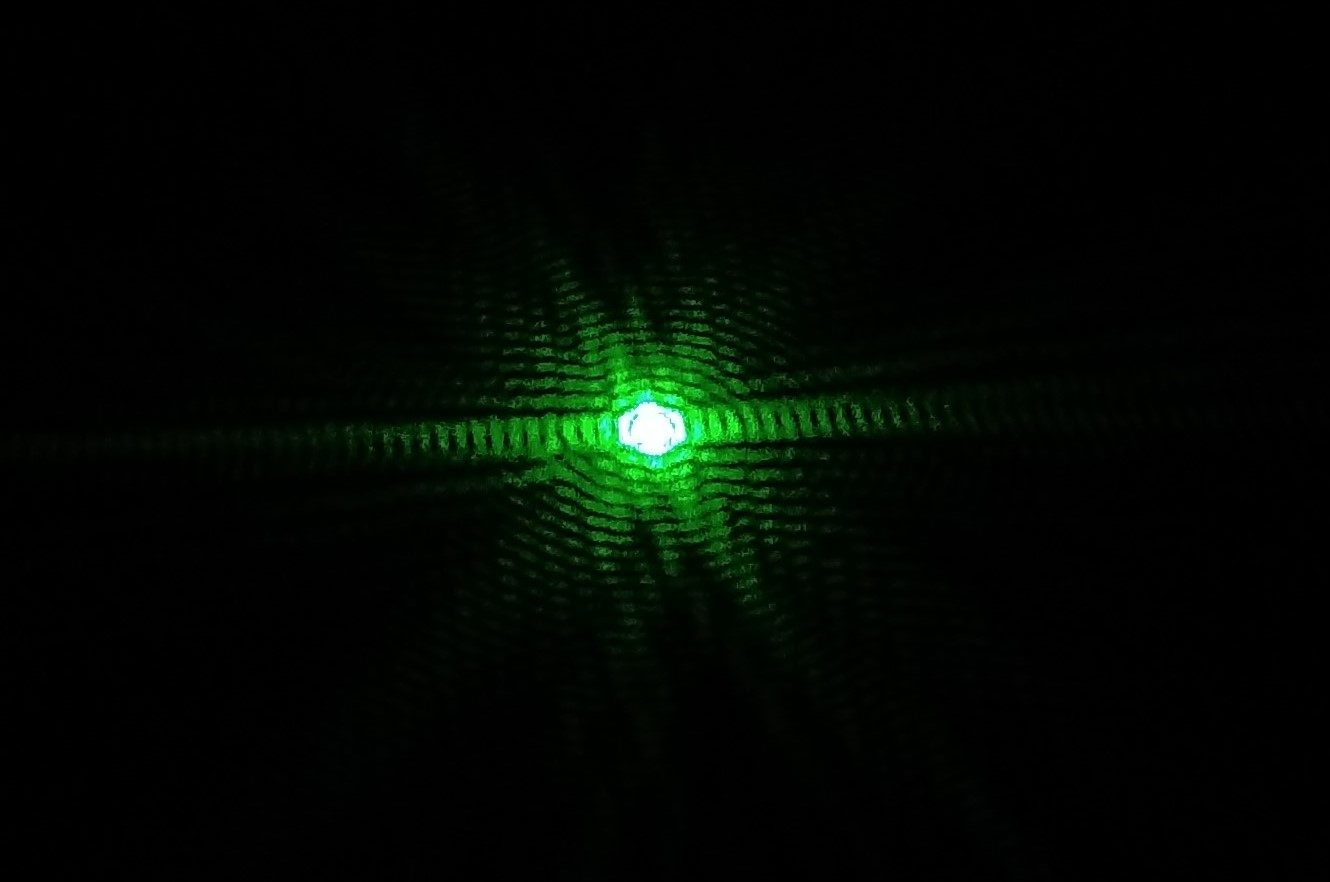
\includegraphics[scale=0.18]{hole.jpg}
\end{center}


\hfill\break
\hfill\break
\section{Summary}
In Lab 4 of Physics 391, we measured the thickness of several objects on the micron scale by using the diffraction and interference properties of light. The result of the measurements is generalized in the table in section 4.3.1 in this text. We also use the Michelson interferometer to measure the thickness of a cover glass and a microscope slide. And lastly, we observe several patterns generated by the illuminated square mesh, helical lamp filament, and a circular hole in an aluminum foil. 





\newpage
\section{Experiment Data}
\begin{center}
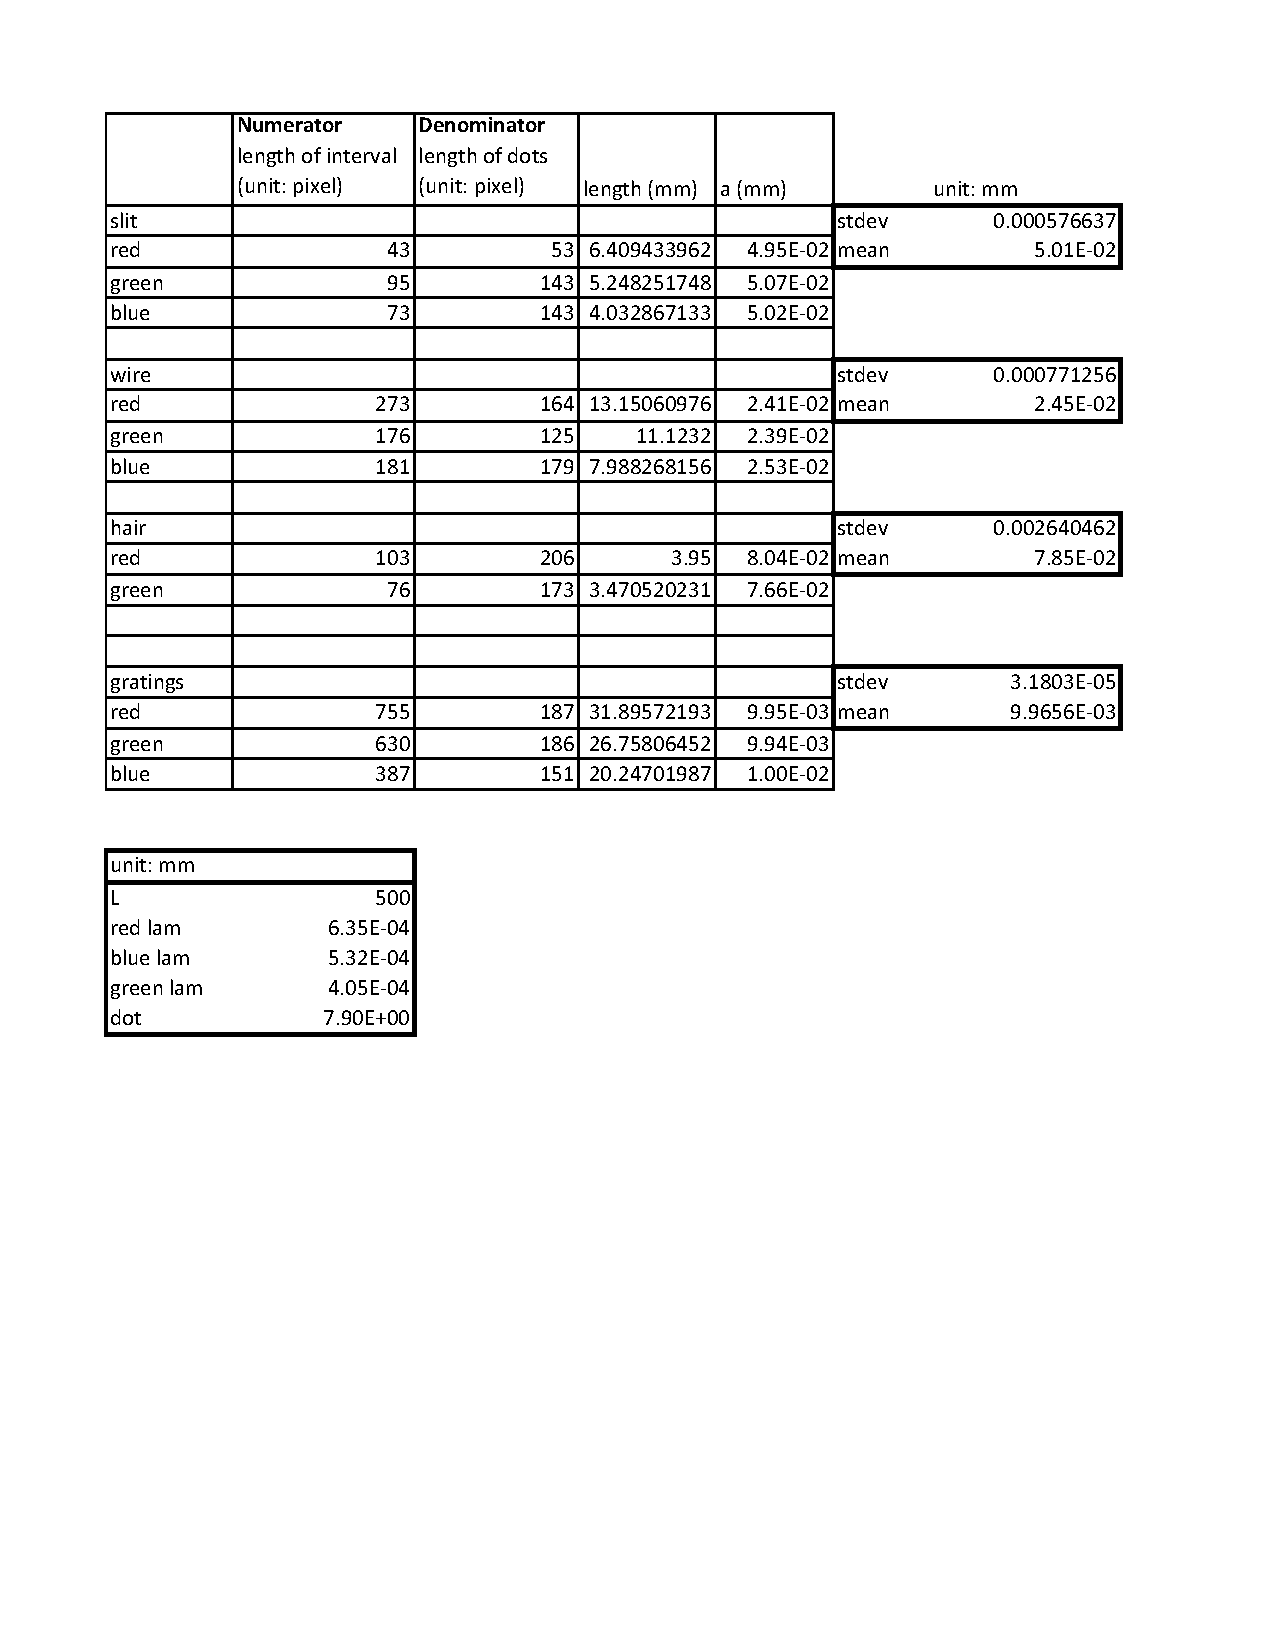
\includegraphics[scale=0.69]{lengths.pdf}
\newpage
\includegraphics[scale=0.69, page=2]{lengths.pdf}
\end{center}
\end{document}